\documentclass{beamer}
\usepackage{amsmath,amsthm,ifthen}
\usepackage{uofmtheme}
\title{Interfaces Introduce Extension}
\author{John Chilton}

\begin{document}
\frame{\titlepage}

\section{Introduction}
\subsection{Overview}
\frame{
\frametitle{Interfaces Extension (1 / 3)}
\begin{block}{Operation Creation}
Allows developers to annotate fields of the service implementation class as implementing plain old Java interfaces on behalf of the service. The extension will automatically create matching grid operations and implement these via delegation to the annotated object.
\end{block}
}

\frame{
\frametitle{Interfaces Extension (2 / 3)}
\begin{block}{Operation Management}
As interfaces are added, removed, and modified the extension continues to ensure the caGrid service is synchronized with the given interfaces.
\end{block}
Note: The developer may still manually add, implements, and manage other operations.
}

\frame{
\frametitle{Interfaces Extension (3 / 3)}
\begin{block}{Client}
Creates a client class that implements all of these interfaces via delegating method calls to the normal Introduce generated caGrid client. This enables users of the service to program againist the Java interfaces.
\end{block}
}

\subsection{Calculator Example}
\frame{
\frametitle{The Interfaces}
\begin{block}{\ttfamily Adder.java}\ttfamily
package calc;\\
public interface Adder \{ \\
~~int add(int x, int y); \\
~~int add3(int x, int y, int z); \\
\}
\end{block}
\begin{block}{\ttfamily Subtracter.java}\ttfamily
package calc;\\
public interface Subtracter \{ \\
~~int subtract(int x, int y);\\
\}
\end{block}
}

\frame{
\frametitle{The Implementations}
\begin{block}{\ttfamily AdderImpl.java}\ttfamily
package calc;\\
public class AdderImpl implements Adder \\
\end{block}
\begin{block}{\ttfamily SubtracterImpl.java}\ttfamily
package calc;\\
public class SubtracterImpl implements Subtracter  \\
\end{block}
\begin{block}{\ttfamily Calculator.java}\ttfamily
package calc;\\
public class Calculator implements Adder, Subtracter \\
\end{block}
}

\frame{
\begin{columns}
\column{3cm}
Create a calculator service for this example.
\column{7cm}
\begin{center}
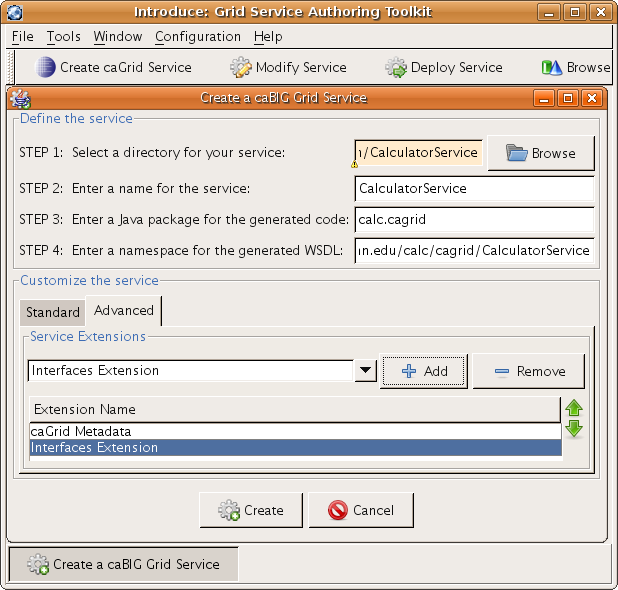
\includegraphics[scale=.30]{images/interfacesCreate.png}  
\end{center}
\end{columns}
}


\section{The Basics}
\subsection{Service Side}

\frame{
\begin{block}{\ttfamily CalculatorServiceImpl.java}\ttfamily
package calc.cagrid.service; \\
~\\
\color{maroon}import edu.umn.msi.cagrid$\hdots$ImplementsForService; \color{black}\\
import java.rmi.RemoteException; \\
~\\
public class CalculatorServiceImpl extends $\hdots$ \{\\
~~public CalculatorServiceImpl() throws $\hdots$ \{\\
~~~~super();\\
~~\}\\
\}
\end{block}
The Interfaces extension added an import to the service implementation file for the annotation \texttt{ImplementsForService}.
}

\frame{
\frametitle{Annotating the Adder Interface}
\begin{block}{\ttfamily CalculatorServiceImpl.java}\ttfamily
\color{maroon}import calc.Adder; \\
import calc.AdderImpl; \\
\color{black}
$\hdots$ \\
public  class CalculatorServiceImpl $\hdots$ \{\\
\color{maroon}~~@ImplementsForService(interfaces=\{"calc.Adder"\}) \\
~~Adder adder;\color{black} \\
~\\
~~public CalculatorServiceImpl() $\hdots$ \{\\
~~~~super();\\
~~~~\color{maroon}adder = new AdderImpl();\color{black}\\
~~\}\\
\}
\end{block}
}


\frame{
\begin{columns}
\column{3cm}
Upon adding the jar file containing the calculator example to the project and saving the service in Introduce, the \texttt{Adder} operations are automatically created and implemented.
\column{7cm}
\begin{center}
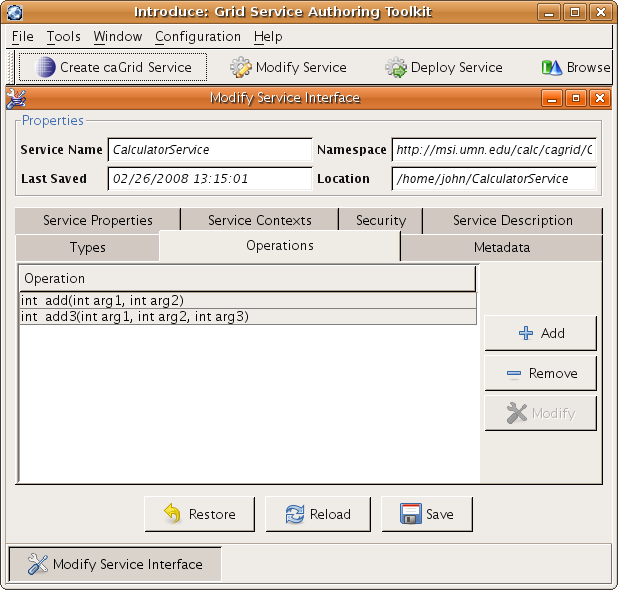
\includegraphics[scale=.30]{images/interfacesSave1.png}  
\end{center}
\end{columns}
}

\frame{
\begin{block}{\ttfamily CalculatorServiceImpl.java}\ttfamily
$\hdots$ \\
public class CalculatorServiceImpl $\hdots$ \{\\
~~@ImplementsForService(interfaces=\{"calc.Adder"\}) \\
~~Adder adder; \\
~\\
~~\color{maroon}\small@ImplementsForService\normalsize (interfaces=\{"calc.Subtracter"\}) \\
~~Subtracter subtracter; \color{black}\\
~\\
~~public CalculatorServiceImpl() $\hdots$ \{\\
~~~~super();\\
~~~~adder = new AdderImpl();\\
~~~~\color{maroon}subtracter = new SubtracterImpl();\color{black} \\
~~\}\\
$\hdots$
\end{block}
}

\frame{
\begin{columns}
\column{7cm}
\begin{center}
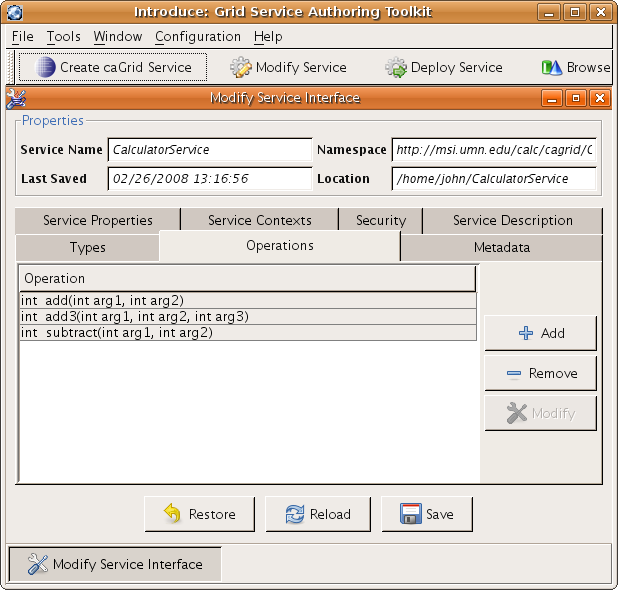
\includegraphics[scale=.30]{images/interfacesSave2.png}  
\end{center}
\column{3cm}
Resaving causes the new operation corresponding to \texttt{Subtracter} to be created.
\end{columns}
}

\frame{
The developer can add interfaces, remove interfaces, and change the field that implements an interface and the caGrid service operations and implementations will be modified accordingly next time the service is saved in Introduce.
}

\frame{
\begin{block}{\ttfamily CalculatorServiceImpl.java}\ttfamily
public  class CalculatorServiceImpl $\hdots$ \{\\
~~\color{maroon}@ImplementsForService(interfaces=\{ \\
~~~~~~~~~~~~~~~~~~~~~"calc.Adder","calc.Subtracter"\}) \\
~~Calculator calculator; \\
~\\
~~\color{black}public CalculatorServiceImpl() $\hdots$ \{\\
~~~~super();\\
~~~~\color{maroon}calculator = new Calculator(); \\
~~\color{black}\}\\
$\hdots$
\end{block}
}

\frame{
\begin{columns}
\column{3cm}
After saving, all of the operations are still there though their implementations have changed.
\column{7cm}
\begin{center}
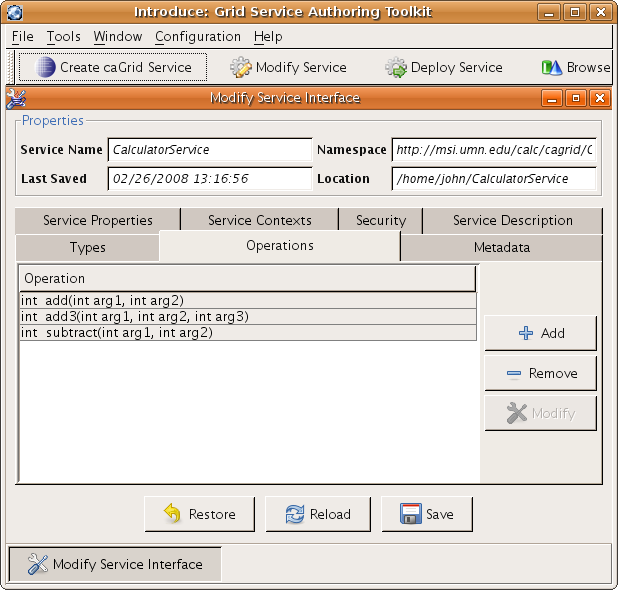
\includegraphics[scale=.30]{images/interfacesSave2.png}  
\end{center}
\end{columns}
}

\frame{
The developer can make changes to the interfaces themselves and replace the corresponding jars. After restarting Introduce and saving, the service operations and implmentations will again adapt to the interface changes.

\begin{block}{Warning}
After replacing jars in a service's \texttt{lib} directory, Introduce \textbf{must} be closed and reopened before saving the service.
\end{block}
}

\frame{
\frametitle{Make Some Changes}
\begin{block}{\ttfamily Adder.java}\ttfamily
package calc;\\
public interface Adder \{ \\
~~int add(int x, int y, String ticket); \\
~~int add3(int x, int y, int z, String ticket); \\
~~int addArray(int[] xs, String ticket); \\
\}
\end{block}
\begin{block}{\ttfamily Subtracter.java}\ttfamily
package calc;\\
public interface Subtracter \{ \\
~~int subtract(int x, int y, String ticket);\\
\}
\end{block}
}

\frame{
\begin{columns}
\column{3cm}
After replacing the jar, restarting Introduce, and saving the service, the new operations will appear.
\column{7cm}
\begin{center}
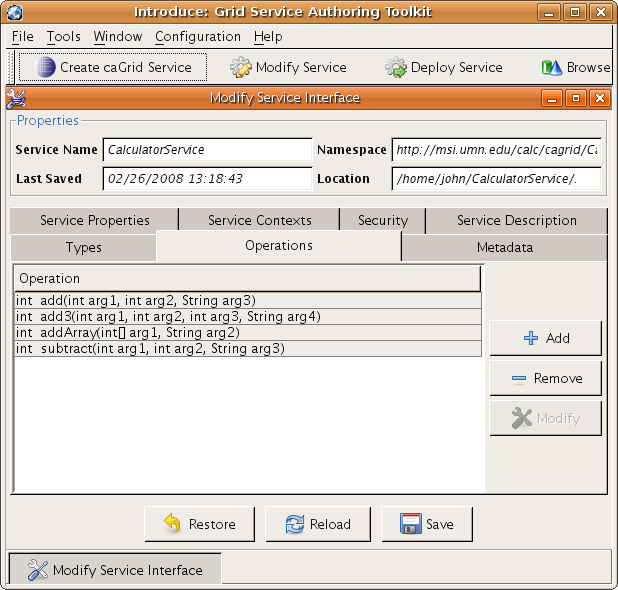
\includegraphics[scale=.30]{images/interfacesSave3.png}  
\end{center}
\end{columns}
}

\subsection{Client Side}
\frame{
\frametitle{The Interfaces Client}
The extension creates a client class that implements all of these interfaces via delegating method calls to the Introduce generated caGrid client.
\begin{block}{\ttfamily CalculatorServiceInterfacesClient.java}\ttfamily
public  class CalculatorServiceInterfacesClient\\
~~~~~~implements calc.Adder, calc.Subtracter \{\\
~~$\hdots$ \\
\}
\end{block}
}

\frame{
\frametitle{The Interfaces Client Constructors}
The Interfaces client can be constructed using any of the argument combinations permitted by the Introduce generated client class or using an Introduce generated client instance directly.
}

\frame{
\begin{block}{\ttfamily SomeClass.java (Pseudocode)}\ttfamily
\frametitle{Programming Againist an Interface}
\textit{// A class that uses an Adder to do work}\textnormal \\
public class SomeClass \{ \\
~~Adder adder; \\
~~public static SomeClass create() \{ \\
~~~~if(runningOnHost()) \\
~~~~~~\textit{// Set adder to a calculator} \\
~~~~else \\
~~~~~~\textit{// Set adder to a interfaces service client} \\
~~\} \\
~~$\hdots$
\end{block}
Effect is even cleaner using a dependency injection framework, such as Spring.
}

\frame{
\begin{block}{\ttfamily AdderTestCase.java}\ttfamily
\frametitle{Testing Againist an Interface}
public class AdderTestCase \{  \\
~~public void testAdder(Adder adder) \{ \\
~~~~assert 2 == adder.add(1,1); \\
~~\} \\
\}
\end{block}

Can use (mostly) the same code to test deployment as server side implementation.
}

\frame{
\frametitle{Refactoring}
As of Eclipse 3.2, you may create ``scripts'' out of your refactorings and distribute them. This has the potential to reduce the amount of work your users have to do if you happen to refactor the underlying interfaces and your users are programming againist these interfaces.
~\\
~\\
If you happen to be a consumer of your own services and your client project references your service project, Eclipse should do all of the refactoring of your client code automatically.
}

\section{Going Further}
\subsection{Interface Annotations}
\frame{
\begin{block}{Customizing The Operations}
A developer can customize certain aspects of generated operations via annotations on the underlying Java interface.
\end{block}
In most cases interfaces should work out of the box and these annotations are entirely optional as long as Introduce knows about the referenced types and the method names are unique and valid operation names.
}


\frame{
\frametitle{Method Overloading (1 / 3)}
\begin{block}{\ttfamily Adder.java (Invalid)}\ttfamily
package calc;\\
~\\
public interface Adder \{ \\
~~int add(int x, int y); \\
~~\\
~~int add(int x, int y, int z); \\
~~\\
~~int add(int[] xs); \\
\}
\end{block}
Invalid interface for annotating a caGrid service with, resulting operation names must be unique!
}

\frame{
\frametitle{Method Overloading (2 / 3)}
\begin{block}{Adder.java}\ttfamily
package calc;\\
\scriptsize import edu.umn.msi.cagrid.introduce.interfaces.client.\normalsize GridMethod; \\
public interface Adder \{ \\
~~int add(int x, int y); \\
~~\\
~~\textit{// Use add3 as operation name instead}\\
~~@GridMethod(operationName="add3")\\
~~int add(int x, int y, int z); \\
~~\\
~~@GridMethod(operationName="addArray")\\
~~int add(int[] xs); \\
\}
\end{block}
}


\frame{
\frametitle{Method Overloading (3 / 3)}
\begin{block}{Some client code}\ttfamily
~~void foo() \{ \\
~~~~CalculatorServiceInterfacesClient client;\\
~~~~$\vdots$ \\
~~~~\textit{// Client has overloaded methods, even though \\
~~~~// underlying grid service cannot.}\textnormal\\
~~~~int sumOf2 = client.add(1,2); \\
~~~~int sumOf3 = client.add(1,2,3); \\	
~~~~int sumOfArray = client.add(new int[]\{1,2\}); \\
~~~~$\vdots$ \\ 
~~\}
\end{block}
}

\frame{
\frametitle{XML Type Disambiguation (1 / 4)}
\begin{block}{\ttfamily Adder.java}\ttfamily
public interface Adder \{ \\
~~int add(int x, int y, String ticket); \\
\}
\end{block}
The extension must guess what XML type the developer wants \ttfamily{ticket}\sffamily{ to map to, both of the types }\ttfamily{string}\sffamily{ or }\ttfamily{anySimpleType}\sffamily{ from the W3C XML Schema namespace map to }\ttfamily{java.lang.String}.
}


\frame{
\frametitle{XML Type Disambiguation (2 / 4)}
Other out of the box ambigous types:
\begin{itemize}
 \item \texttt{java.lang.String} could map to \texttt{string}{* or }\texttt{anySimpleType}.
 \item \texttt{byte[]} could map to an array of \texttt{byte}s, a \texttt{hexBinary}, or a \texttt{base64Binary}*.
 \item \texttt{byte[][]} could map to an array of \texttt{hexBinary}s or \texttt{base64Binary}s*.
\end{itemize}
* indicates the Interfaces extension default choice.
}

\frame{
\frametitle{XML Type Disambiguation (3 / 4)}
You can override the default XML mapping on parameters as follows.
\begin{block}{\ttfamily Adder.java}\ttfamily
\scriptsize import edu.umn.msi.cagrid.introduce.interfaces.client.\normalsize GridParam; \\
public interface Adder \{ \\
~~int add(int x, int y, \\
~~~~~~@GridParam(\scriptsize namespaceURI="http://www.w3.org/2001/XMLSchema"\normalsize, \\
~~~~~~~~~~~~~~~~~\scriptsize localPart="anySimpleType"\normalsize) \\
~~~~~~String ticket); \\
\}
\end{block}
}



\frame{
\frametitle{XML Type Disambiguation (4 / 4)}
\begin{block}{\ttfamily Foo.java}\ttfamily
\scriptsize import edu.umn.msi.cagrid.introduce.interfaces.client.\normalsize GridResult; \\
public interface Foo \{ \\
~~@GridResult(\scriptsize namespaceURI="http://www.w3.org/2001/XMLSchema"\normalsize, \\
~~~~~~~~~~~~~~\scriptsize localPart="hexBinary"\normalsize) \\
~~byte[] foo(int x); \\
~~\\
~~@GridResult(\scriptsize namespaceURI="http://www.w3.org/2001/XMLSchema"\normalsize, \\
~~~~~~~~~~~~~~\scriptsize localPart="byte"\normalsize) \\
~~byte[] foo2(int x); \\
\}
\end{block}
Note: The extension determines if the mapped type should (as in \texttt{foo2}) or should not (as in \texttt{foo}) be an array automically.
}

\frame{
\frametitle{Additional Annotation Options}
\texttt{GridParam} can also be used to set the name of the parameter with the \texttt{name} field. 
~\\
~\\
All three annotations have a \texttt{description} field which can be used to set a description for the method, parameter, or result respectively.
~\\
~\\
\texttt{GridMethod} has a \texttt{boolean} field \texttt{exclude} that can be used to prevent the creation of operation for that method. If the corresponding method is then called on the Interfaces client, a \texttt{java.lang.UnsupportOperationException} is thrown.
}

\subsection{Exception Handling}

\frame{
\frametitle{Exception Handling}
The Introduce generated client code only throws \texttt{RemoteException}s. These could be because the delegated method threw an exception or because of some other issue such as a connection problem. If the interface method permits a \texttt{RemoteException} to be thrown, this exception will be thrown as is, if not the exception is wrapped in a runtime exception first.
~\\
~\\
Essentially, the fact an exception is thrown by the underlying implementation survives and reaches the client, but the type and content of the exception will likely not.
}


% \frame{
% \begin{block}{Foo.java}\ttfamily
% public interface Foo \{\\
% ~~public void foo1() throws Exception; \\
% ~~public void foo2() throws IOException; \\
% ~~public void foo3() throws RemoteException; \\
% ~~public void foo4() throws FileNotFoundException; \\
% ~~public void foo5();\\
% \}
% \end{block}
% If any exception is thrown while executing foo1, foo2, or foo3 on the service side, it will come back and be thrown out of the client method as a RemoteException. If RemoteException is thrown by  foo4 or foo5 the RemoteException will be wrapped in a runtime exception. foo4 of the interfaces client will never actually throw a FileNotFoundException.
% }


\end{document}
